\documentclass[10pt,twocolumn]{article}

% use the oxycomps style file
\usepackage{oxycomps}

% usage: \fixme[comments describing issue]{text to be fixed}
% define \fixme as not doing anything special
\newcommand{\fixme}[2][]{#2}
% overwrite it so it shows up as red
\renewcommand{\fixme}[2][]{\textcolor{red}{#2}}
% overwrite it again so related text shows as footnotes
%\renewcommand{\fixme}[2][]{\textcolor{red}{#2\footnote{#1}}}

% read references.bib for the bibtex data
\bibliography{references}

% include metadata in the generated pdf file
\pdfinfo{
    /Title (On a Roll! Development of a Dice-Based Arcade Fighting Game)
    /Author (Max Cheng)
}

% set the title and author information
\title{On a Roll! Development of a Dice-Based Arcade Fighting Game}
\author{Max Cheng}
\affiliation{Occidental College}
\email{acheng2@oxy.edu}

\begin{document}

\maketitle

\section{Abstract}

This paper will cover the development process and background  of the vertical slice of On A Roll, a simple, isometric fighting game using roguelike elements to create a play experience similar in scope and gameplay to that of an arcade game. There exist a variety of games that make use of different individual features that On a Roll comprises, as well as a variety of implementation options for the presented functionalities. The design process and final architectural decisions were made and implemented based on factors including personal goals for the project, intended scope of gameplay, and feasible development time. Similarly, playtesting evaluation metrics were determined with consideration to player experience versus the stated goals for the project, guided towards qualitative feedback that would be the most useful to incorporate into an ongoing development process.


\section{Introduction and Problem Context}

Video games at this point in time span an impressive range of genres, playstyles, and designs. Games are no longer a category of media broadly constrained to a single kind of consumer, expanding past the notoriety of FPS shooters to invite players to an expansive list of options ranging from story-based narratives, to immersive action games, to complex platforming. For this project, I sought to make a game paying homage to different games that I have loved and have resonated with me, taking an opportunity both to hone my own taste and personal game design sense as well as explore the technical implementation behind a game genre that I have little experience with building.
This game, although perhaps not the most groundbreaking of projects, seeks to unify different mechanics and functionalities from a variety of existing games that I have enjoyed to create a new arcade-style, roguelike-inspired fighting game. The definitions and details of these descriptions are elaborated on in Section 3: Technical Background. My personal design goals are based on aspects of games that I have played that have resonated the most with me, and left me with the most memorable player experience, in conjunction with what I feel would be the ideal player experience based on the scope and design of this particular game. Therefore, there is a special emphasis on a few different aspects:
First, gameplay feel and movement responsiveness. The games that I have often felt I have the most fun with are those where the moment-to-moment gameplay is engaging, where the movement feels satisfying and is fun to interact with even in an empty environment. Games like Dead Cells and Celeste \cite{deadcells} \cite {celeste} are robust and feature well-designed narratives and gameplay, but what fundamentally keeps me engaged with them is simply how fun they feel to control, and how clean their physics interactions are. Second, enemy calibration: This is a vertical slice, but even within the scope of a full game there would not be much in terms of meta-progression or heavily varied mechanics. Thus, to keep things interesting and to maintain a level of difficulty that the player would need to improve their own skills for, the enemy behavior should be complex and varied enough to provide a real challenge. More detailed design choices and goals will be provided in Section 5.1: Design Process, but these are the most important of the issues I hope to address.

\section{Technical Background}
The design of the game with respect to overarching mechanics and the gameplay loop is based on gameplay conventions from the arcade and roguelike genres. Each brings a unique standpoint on the subject of player engagement, and by extension, the notion of "replayability": how inspired a player would be to return to a game and continue playing it even after they have completed a stated main objective.

\subsection{Arcade Games}
Some of the earliest video games, and in particular the earliest prominent multiplayer games, were arcade games—if not strictly games set on arcade machines, games that still featured many of the design tendencies of arcade games. For instance, meta-progression was a rare find in any game throughout the early chunk of their history - in part because the technology was still too limited to fully implement save states, but also (as in the case of arcade games) because players didn't often stick around the same machine for long enough to make significant progress. \cite{arcades} All the progression made in a game had to be done in one sitting, and would be lost the moment a session was closed or abandoned. Arcade-style games as a genre of course do still range in complexity and progression detail, but the crux of the design is the same: beyond simple engagement mechanics like beating a high score, players are engaged and inspired to come back based on their enjoyment of playing the game itself. In addition, this style of game often does not feature an extensive tutorial: typically there will be a brief explanation of how the controls work, and some tip on the objective of the gameplay. Succeeding at a game, however, will more often come down to the player's own skill level and successful mastery of the controls. For example, the game \textit{Tetris} demonstrates a variety of these concepts:
\begin{itemize}
    \item Controls and game objectives are very simple to learn and understand
    \item Progression is limited to the game speed increasing with levels, but the mechanics do not change at any point
    \item There is a scoring system to encourage competitive players to beat different high scores, but no carefully-engineered loop of engagement or focus on "replayability"
    \item Players' ability to succeed at the game depends largely on their own skill with the controls and the mechanics of the game, rather than being one where time invested in a session creates game progression.
\end{itemize}

\subsection{Roguelikes}
Roguelikes are a genre reliant on an element of randomness, notably in the form of procedural generation, as a means of creating variety and diversity in the gameplay experience every time the game is played. In a roguelike, when the player is killed, they are returned to the very beginning of a level, forced to work their way back up from scratch to finally reach the finish. Each time they start or restart, known colloquially as a "run" of the game, randomness may be applied to different factors like terrain, level progression, enemies, weapons, bonuses, and so on. This ensures that although the same fundamental content is being endlessly repeated, the actual details of the gameplay are continually varied enough for the player to need to adapt to and master the controls and mechanics of the game. \cite{roguelikes}The "replayability" factor of a roguelike is driven first by inspiring the player to want to complete a full run and reach the ending, but also by providing continually interesting variations on a game the player will have grown adept with controlling. 


\section{Prior Work} 
Outside of overarching genre categories, there are specific features and examples of playstyles that are exemplified by various existing games, providing a helpful frame of reference in describing particular mechanics of the design. 

\subsection {Hades}
Hades is an isometric, 2.5D roguelike whose gameplay goals are for the player to battle their way out of the Underworld, with assistance from various Greek gods in the form of unlockable effects that modify different aspects of combat. The overall isometric framing of the game, as well as the real-time, hack-and-slash style of combat interactions are aspects that feature in the design for this game. \cite{hades}

If the scope of the project were to be expanded outside that of a vertical slice, the way that Hades handles individual level progression (upon defeating the current level, selecting new 'rooms' with various gimmicks or rewards to continue on through) would be ideal to implement to build a more extended gameplay loop per "run." Hades' method of meta-progression is also well-suited to the style of this game, in that resources collected during gameplay can be used to unlock different weapons and abilities, further increasing the level of variety gained from the game overall.


\subsection {Boomerang Fu}
Boomerang Fu is a cartoony, 3D fighting game meant to be played with a large group of people. The combat is fairly simple, each player having access to a melee and ranged attack, but throughout each round the terrain spawns a variety of power-up options that can be picked up and used by any player. All players start with the same health, attack, and statistics, but the kinds of power-ups obtained can drastically affect abilities and therefore the player's approach to combat in the game. I was most drawn to Boomerang Fu as an example because it pulls from a common pool of powerups, and because no player is granted significant statistical advantage over anyone else due to its nature as a multiplayer game. When playing the game myself, this had the effect of emphasizing each player's personal skill at the game, in contrast to how many games use differing scales for enemy statistics versus player statistics as a way of ramping in difficulty. \cite{boomerang}

\subsection {Dungeons and Dragons}
Dungeons and Dragons is the most prominent example, but overall the function of many tabletop RPG games uses the rolling of dice to determine different outcomes in the game. Regardless of how well-equipped a player might be, they are still subject to the restrictions of the dice outcome for any given situation. Similarly, perfect balance of randomization from run to run is not my goal with development - certain situations have the chance to be much more challenging than others, forcing the player to be more resourceful and tactical with their approach to the combat. The video game Mosa Lina \cite{mosa} shares a similar feature, where not every randomly generated toolset will actually be able to solve the problem at hand.

From a design and immersion standpoint, the Dungeons and Dragons convention of splitting characters into different "classes" to determine their statistics and abilities was also a feature used to inspire the character design of the player and enemy abilities. This was helpful in adding variety to the enemy behaviors, creating a mix of enemies that the player may have to interact with and balance against at any given point. \cite{dnd}



\section{Methods}

\begin{figure}
    \centering
    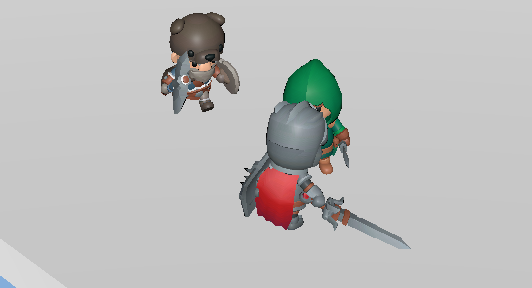
\includegraphics[width=.95\linewidth]{fight.png}
    \caption{
        A somewhat poorly-framed action shot (It's hard to play and screenshot at the same time!)
    }
    \label{fig:first-page}
\end{figure}

The methods employed in creating this game can be broken down into two primary components: the design process from start to finish of compiling inspirations, creating an idea, and narrowing scope to an acceptable level for this project; and second, the technical implementation of the more complex game systems. 

\subsection{Design Process}
The design process started with the basic concept of using a dice roll as the triggering mechanism to generate randomness in a roguelike game. I have previously made mostly games in 2D, or very limited 3D, so I came into the process knowing that I wanted to use this process as a means of learning more about 3D motion and development. The best way to unify the two seemed to be some system of real-time combat, which became the basis for the rest of the design.
Initially, I had planned the game to be more faithful to the roguelike genre, with plans for more meta-progression (adding to a player's resources between runs), and more robust levels and progression built into each run. However, considering the time scale available to me for the project and the scope of what would be feasible, a lot of the progression features were abandoned. At this point, the switch to a more arcade-style game grew more appealing: there was no need to implement complex progression, but extended gameplay was still possible, especially using the natural randomized mechanics of the dice to keep play varied and interesting.

\subsection{Gameplay}
The game starts with the player clicking to roll a set of three dice. The first corresponds with the number of enemies that will be present, the second with the number of power-ups that the player will have available to them, and the third with the number of power-ups that the enemy team will have available to them. The types of enemies generated are randomized internally, attempting first to generate at least one Barbarian enemy and then at least one Rogue enemy. Subsequent enemy generations are entirely randomized. The power-up pools given to both the player and the enemy are also randomized internally, with no limitations on what can generate for either. The player can use their power-ups at any time, with no limits on overlapping power-ups with the exception that the same type of power-up will not stack with itself (for example, a speed boost power-up cannot be triggered if a speed boost is already active). The gameplay goal is to eliminate every enemy through real-time combat. 

The player is a character of the Knight class who is able to jump, attack, dash, and block as its basic movement functionalities. Their goal is to eliminate all present enemies in order to advance to the next "level" of the game, where the previously described gameplay loop repeats itself (at least for the scope of this vertical slice). The player's statistics, including health, speed, and attack damage, are considered the default statistics. Different enemy types will have modified statistics relative to the default.

There are two types of enemies: The Barbarian and the Rogue. 
The Barbarian aligns closely with typical 'tank' classes, equipped with more health but lower speed. The Barbarian's attacks will also deal more damage but take a longer time to execute, opening dodging and interrupting as viable strategies. The Barbarian's attacks, as a heavy attack, cannot be blocked by the player's shield. 

The Rogue has somewhat the inverse, having default health but a very high speed and a lower hit damage. The Rogue operates by chasing into range to attack the player, then quickly retreating out of the player's range before it can receive retaliation. The Rogue's attacks can be blocked by the player's shield.

When multiple enemies are present, they all share the same pool of available power-ups. If one entity consumes a power-up, it is consumed for all enemy entities. The benefits of the power-up also only apply to the enemy that triggered its consumption, not all enemies at once. 

There are 5 power-ups available: invulnerability, speed boost, unblockable attacks, healing, and damage boost. The same pool of power-ups applies to both the player and the enemies, and function identically regardless of the entity it applies to. Of the five:

\begin{enumerate}
    \item Invulnerability: absorbs one attack of any kind and prevent it from damaging the user. If an invulnerability shield is attacked by an unblockable attack, therefore, the shield will still absorb the hit and disappear after.
    \item Speed boost: upon activation, boosts the movement and attack speed of the entity for 5 seconds. The speed boost is applied as a flat increase to the entity's current speed parameter, regardless of relation to the default speed. 
    \item Unblockable: attacks allow the entity's weapon to hit regardless of if the attack was blocked, for the next attack after the power up is activated. If the next attack was not attempted to be blocked, the power-up is consumed regardless. 
    \item Healing: restores 20\% of the entity's maximum health immediately upon use.
    \item Damage boost: upon activation, boosts the attack damage of the entity by a flat increase for 3 seconds. 

\end{enumerate}

\subsection{External Resources}
Preparing to begin the development process involved research of different possible algorithms and implementations of the technical features I wanted to add, as well as exploration for potential assets that could be employed as a way of creating a better sense of worldbuilding and immersion. 

A majority of the architecture and basis for the code used in my movement controller and enemy behavior decision-making comes from tutorial series \citetitle{tutorial} \cite{tutorial}. Various aspects and implementations vary, of course, to suit the needs of this specific project and the assets used, but the general structure is about the same. 


\subsection{Movement Controller}
The movement controller for the player is built using technically a state machine algorithm. The core foundation of implementing different independent states (in this case, different possible move sets: "idle", "run", "attack", "dead", and so on) is present, but unlike a fully traditional state machine the states themselves do not contain much by way of transition logic to other states. Barring "forced" states that are reactive to the external environment, like staggering upon a hit, having an attack parried, or being killed, all decisions about what state to select next are dependent upon the player's input. Attempted inputs are run through a series of checks to determine the actual returned action: if multiple inputs are pressed for a single frame, the inputs need to be sorted by relevance, if the player has attempted to use a move that they are unable to execute (for example, attempting to use a power-up when there are none left), or if a more relevant move is currently being executed (for example, if the player is in the middle of being parried, their attempts to attack will not register valid inputs). Individual states occasionally contain parameters for actions that need to be taken upon entering or exiting their own state, but do not govern which state to enter next. If the player has not entered any input and no other state is currently taking precedent, the game will default to an "idle" state for the player.

Although the transitional aspects of the state machine algorithm are not well-preserved for the player input controller, I still felt it was the most appropriate framework to apply. First, the organization of different player actions into disparate, easily manageable states makes scaling the project much easier, and offers a good foundation for future work that could require more complex transition logic. Secondly, the enemy characters use overlapping functionalities for their own movement systems. Maintaining the same architecture throughout the project was a more streamlined, logical solution than to attempt applying different architectures for very similar end results

There also exists a 'resources' check layer that manages health levels and power-up functionalities. Successful attacks decrease the entity's health, and when health reaches zero the entity is forced into the 'death' state. The implementation of the power ups is fairly simple, first checking that a power-up can be used and which one should be triggered. Because each of the powerups simply alters the status of existing interactions, no new frameworks or state switching is necessary, only altering of certain parameters.

\subsection{Enemy Behavior}
The enemy behaviors and decision-making do follow a more traditional state machine model. Following overarching behavior loops based on the type of enemy, each individual state contains direct instructions for which state to transition to next based on various factors like distance from the player, number of successful attacks, and whether any enemy or player powerups are active. All enemies, unless in the "evade" state, will default to "pursue" anytime the player is further than the enemy's personal attack radius. If the player has activated an offensive powerup:  damage boost, unblockable, or speed boost power-up, all enemies will attempt to evade until the duration of the power-up has elapsed. When any enemy is at or below 20\% of its maximum health, it will trigger a power-up for itself, if available, but gives priority to whichever living enemy entity currently has the least health. 

The Barbarian enemy will pursue the player until they are within the Barbarian's attack radius, and then continues attempting attacks until it has successfully hit the player three times. After the third hit, the Barbarian will evade and retreat a short distance before moving to pursue the player again. If the player is at or below 30\% health and within a certain radius (wider than the Barbarian's attack radius), the Barbarian will attempt to activate an offensive power-up. 

The Rogue enemy pursues the character until they are within the Rogue's attack radius, but only attempts to land one successful attack before retreating to a fairly distant "evade" from the player. The Rogue will not attempt to activate a power-up unless the player is at or below 15\% health and within its allotted radius.


\subsection{Incorporating Feedback}

When creating a user-facing product, it is especially important to consider actual user feedback and to understand the ways that people interact with the product, and then use that information to continually redesign and improve. The influence of feedback in this project was in two major areas: 

First, the feedback received from peers during the design and initial development phases. Both form feedback from in-class presentations, as well as more individual discussions with peers on the design process and my goals for the project were very influential in shaping the details and scope of the game. Some of the changes made in response to feedback, most notably in regards to shifting from a pure roguelike to more of an arcade game, have already been discussed above. These conversations were helpful in getting me to identify the exact mechanics of the game and their interplay, and then in reshaping the overall style and genre of the game to suit the needs of the gameplay I was creating. Some amount of preliminary development had of course happened by the time I shifted focus, but repurposing the same base implementations to a different end was not a difficult shift.

Second, player feedback was crucial to understanding the actual game experience users were having, and seeing how it did or did not fit in with my own goals and experiences with the game. Feedback was structured to reflect a holistic experience, but also provide more targeted input on areas that I had particular goals for, such as movement. Additionally, an important consideration when collecting feedback for games is who the intended audience is. Unlike with a general-purpose website or app, the game does not necessarily need to be readable and with a tutorial-level interface for any possible user. Failsafes should of course be present, but it would be safe to assume that someone opening my game was at least generally familiar with video games and how they operate. A majority of my playtesting group did fall into this category and was already comfortable with the functions of video games. The question of audience is also good to account for when considering what feedback to build off of, and what feedback may be less relevant. If someone outside the target audience for the game reports having a less amicable experience, or if they suggest changes that would alter more fundamental aspects of the game, the feedback is less immediately applicable to a new iteration of the product. All feedback is still useful, but not all feedback needs to receive equal response.

\section {Evaluation Metrics}
Considering the original stated project goals, this project can be evaluated through the following objectives:
\begin{itemize}
    \item Successful implementation of core game mechanics
    \item Incorporation of quantitative and qualitative feedback in service of original design goals
    \item Players have a fun and enjoyable gameplay experience
    \item Personal understanding of implementation, mechanics, and features
\end{itemize}

The first of these metrics is important for fairly obvious reasons, to evaluate a game the game must exist in the first place. This objective is limited in scope to the mechanics themselves rather than a catch-all for the many details of the game, as aspects such as user experience and other kinds of polish will be reflected more thoroughly with player feedback. 

The sections on feedback are split into feedback that was iterated upon versus players' final impressions of the game once the point of receiving constructive feedback had elapsed. The former goal takes into consideration player feedback as an ongoing, collaborative process, and thus judges the degree to which feedback was both useful and then incorporated into the design and mechanics of the game. 

On the other hand, players' final impressions of the game when they played is valuable for understanding the success of the final product (as opposed to a work in progress seeking guidance). The player experience thus covers how players felt about the mechanical interactions and technical gameplay, as well as a level of product polish, detailing, and user interfacing. 

Finally, though perhaps a less conventional project goal, a personal evaluation of my own understanding of the implementations and techniques. In accomplishing the project, of course, it is expected I would learn how it works, however I did set one of my original project goals as being able to learn and dissect the functions of larger, more complex machine models such as that of a combat game. When additionally considering that this game was not intended to be necessarily groundbreaking or a major innovation in the field, the inspiration and benefits of tackling this project have definitely been (and stayed consistent with) fostering my own ability to utilize and later expand upon implementations.

I do believe these metrics are an accurate summary of the project's original goals, however I recognize that they are largely subjective and/or qualitative and thus would prove difficult to evaluate consistently. Player feedback and satisfaction can be evaluated, even if not numerically, by having the same people playtest more than once, incorporating their suggestions in between and rating their reactions to the different designs. 

\section {Results and Discussion}
Based on the criteria above and the discussion of results in this section, I believe the project achieves a majority of the stated project goals. The largest detractor from me would probably be a lack of polish and friendly user experience when playing the game, as details had definitely been sacrificed for functionality at various points and there was not time to reinstate or further develop a better user interface.

\subsection{Objective 1}
The core mechanics and system interactions of the game have been successfully implemented, as detailed in the above 'Methods' section.

\subsection{Objective 2}
In gathering user feedback, I elected not to use numerical scales. Although numerical data is convenient in that it is easy to compile and visually analyze, I saw two main issues that pointed to numerical results as negligible: Firstly, not every player will have the same understanding of what the numbers on the scale mean. Of course the lowest number generally means 'bad' while the highest means 'very good' is predictable, but players' personal numerical standards for quality are inconsistent and therefore would not provide me substantial information. Secondly, the purpose of this stage was to collect actionable feedback and suggestions that could be taken as guidance in the process of game development, and numerical results fundamentally are unable to offer that level of specificity. Knowing whether someone thought the movement felt good is nice, but if they provide feedback that reactions upon being hit should be more drastic, the usefulness of this second statement is not at all affected by their numerical ranking of its success. 

That said, a majority of the responses received were still not deeply insightful. I was also hesitant to ask too many guiding questions in soliciting feedback, as I did not want my phrasing or delivery of a question to influence how a player experienced and understood the game. Several applicants did note that the original balance of enemy health statistics, as well as the values of bonuses granted by power-ups, felt uneven in favor of the enemies. The new values detailed in this document reflect an updated, more agreeable set of conditions both for power-ups and the capacities of the enemy entities, and playtesters who originally rated these statistics as unbalanced had a more positive reception when testing again following the implemented changes.

Somewhat unfortunately, I did receive a number of reviews that judged it would be better if more fundamental aspects of the game changed. These were not viable responses for this project firstly because the statements in question could not be directly applied as feedback to the existing system, but also because they represented typically different games entirely. My goal was to create a fun and engaging game within the previously established genre boundaries, so suggestions that would begin transgressing such boundaries would have been difficult to incorporate at that stage. For example, a participant at one point suggested that the game be made in 2D rather than 3D, which would not have been paritcularly viable. 

\subsection{Objective 3}
For the final evaluation, a numerical scale was once again not provided by default, but participants were welcome to declare a number of their satisfaction if they so pleased. The comments received seemed to be generally enjoying the combat the most when asked about the game as a whole, but felt that a full polish layer and quality of user experience were somewhat lacking. 

\subsection{Objective 4}
Finally, for my personal evaluation I will consider:
How comfortable do I feel using Godot, as a new engine? Compared to Unity? How well do I feel I have grasped the algorithms used, and to what extent do I feel I would be able to apply or expand upon them in the future? Within the context of games? Outside of it? Would I be able to recreate the features of this game on my own for a different project, without necessarily any of the guidance received here?

I can confidently say I feel that I have succeeded in the final objective. My understanding of Godot feels comprehensive enough to serve as a jumping-off point for the basics of most games I would want to make or would be interested in, particularly in 3D which I had not had previous experience with, even in Unity. My understanding of the node tree system and the connections between different states, screens, and scripts is far more robust, and I am able to both understand it and explain it to others in a way I would not have before. The project has also made me more perceptive of similar implementations or developmental roadblocks I see in other games, far more deeply appreicating the various moving parts and calculations involved in even the simplest motion. I believe I would definitely be able to continue this project if necessary, and could implement similar algorithmic decision-making unguided for necessary situations. Although I leaned heavily on the guidance of the tutorial project in the beginning of the process, the work necessary to separate the code "out of the box" into what was an wasn't usable for me, and why, was a deeply educational experience.

\section{Ethical Considerations}
The foremost ethical considerations for this project would likely be a matter of accessibility, particularly for players with physical disabilities or otherwise limited movement control in some way. Because real-time combat, especially of this variety, depends largely on reaction speed and ability to enter inputs at specific times, it would be difficult to adapt a more accessible solution. One potential option would be to slow movement of all entities, resulting in a less snappy, active game feel but demanding much less strenuous engagement for players who may have trouble with the input speed or with reacting to the events on the screen. 

There are also issues of representation and inclusion. The assets I am using for the characters were from a free online source, and though stylized and "cartoony" it stands that the three characters I am using do not offer a significant range of diversity. All three are some level of white-passing, and only the "Rogue" sprite is female-aligned. Even in the case of the rogue, the presence of the hood makes it difficult to discern the gender. \cite{ethics} There has been research into how players feel their on-screen avatars do, to some extent, embody them as people. In providing only one character design option to the player, they may feel misrepresented or uncomfortable with the racial and gendered connotations of the "Knight" character. If the game were to be expanded in scope, including more variety in all humanoid assets would be an important change to consider, and to make active effort to seek out or design assets that include a broader range of diversity.



\appendix
\section{Replication Instructions}
This project was developed using the Godot v4.2.2 (stable) release, with support from free assets and art acquired online. To replicate and execute the code, download the full 'project code' folder to the local machine, and select the folder to be opened as a new Godot project when prompted. Godot is not the most back-compatible language, but any iteration of Godot above 4.0 should remain functional.

\section{Architecture Overview}
Within the Godot project, larger containers and behavior models are saved each as their own "scene" file that is then imported under whatever base model needs to be used. The state machine operates by representing each state as a physical child node under the 'Model' scene, attaching its behavior directly to the child node. The 'scripts' folder contains all necessary game scripts. Moves, attacks, weapons, and so on are all written as extensions of base versions of each class, to make scaling up easier and smoother. The architecture of the state machine is as follows. 
\begin{figure}
    \centering
    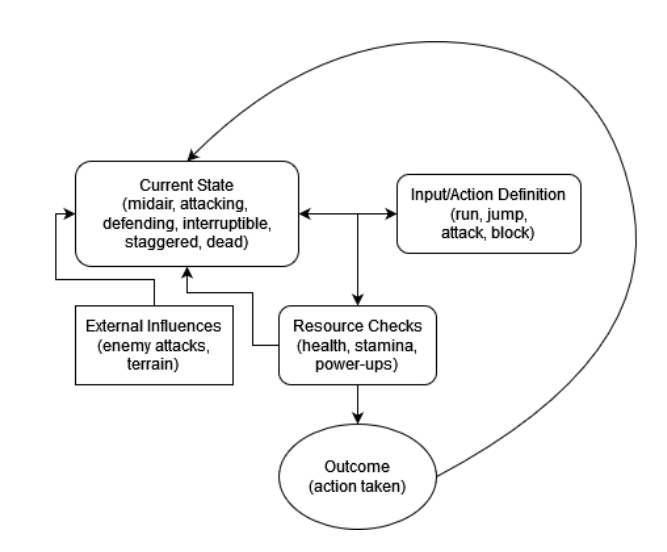
\includegraphics[width=.95\linewidth]{sm.png}
    \caption{
        The organization of the player movement controller state machine.
    }
    \label{fig:first-page}
\end{figure}

\printbibliography

\end{document}
